


\section{设计的主体内容}
在着手进行上机设计之前首先做好大量准备:应熟悉课题,进行调查研究,收集国内、外资料、分析研究;交互界面的设计和实现。

……。
\subsection{系统结构的设计}
……。
\subsection{交互界面的设计和实现}
交互界面的设计应遵循………。
\begin{equation}
        b\approx\frac{L_0}{\rho\tan(\theta_0)+z_0}
\end{equation}
式中,$z_0$为\textit{Goos-Hanchen}位移;$\theta_0$为光波的入射角。

由公式(3-1)可以看出………。
\subsection{线性表的OOP序设计}
计算机内部可以采用两种不同方法来表示一个线性表,它们分别是顺序表示法和链表表示法。

……。

过阻尼响应如图\ref{guozuni}所示。
\begin{figure}[htbp]
\centering

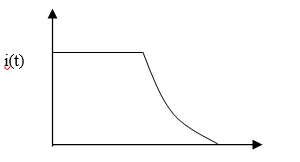
\includegraphics{figure/guozuni.png}
\caption{过阻尼响应}
\label{guozuni}
\end{figure}
\subsubsection{线性表的顺序存储的实现}
……

以上是顺序表的实现过程,第1-16行包含了list类的说明,接下来是成员函数的定义。

……。
\subsubsection{线性表的链表存储的实现}
……

链表的实现包括两个类定义,第一个是link类,第二个是list类。由于一个链表由若干个单独的链结点对象组成,因此一个链结点应当作为单独的link类实现。

……

……